% --- [ Front-end Components ] -------------------------------------------------

\subsection{Front-end Components}
\label{sec:front-end_components}

The front-end module is responsible for converting the input into LLVM IR. Two common scenarios exists, converting binary files (e.g. executables, shared libraries and relocatable object code) and converting source code (e.g. C, Haskell, Rust, …) into LLVM IR. The first scenario is presented in section \ref{sec:design_native_code_to_llvm_ir} and the second in section \ref{sec:compilers}.

% --- [ Subsubsections ] -------------------------------------------------------

% ~~~ [ Native Code to LLVM IR ] ~~~~~~~~~~~~~~~~~~~~~~~~~~~~~~~~~~~~~~~~~~~~~~~

\subsubsection{Native Code to LLVM IR}
\label{sec:design_native_code_to_llvm_ir}

There exist several open source projects which translate native code (e.g. x86 assembly of shared libraries in the PE file format) into LLVM IR. Three such projects have been reviewed in section \ref{sec:rel_work_native_code_to_llvm_ir}, which support different input file formats and machine architectures. These projects may be used as-is by the front-end module to translate low-level source languages into LLVM IR, as illustrated in figure \ref{fig:front-end_binary}.

\begin{figure}[htbp]
	\begin{center}
		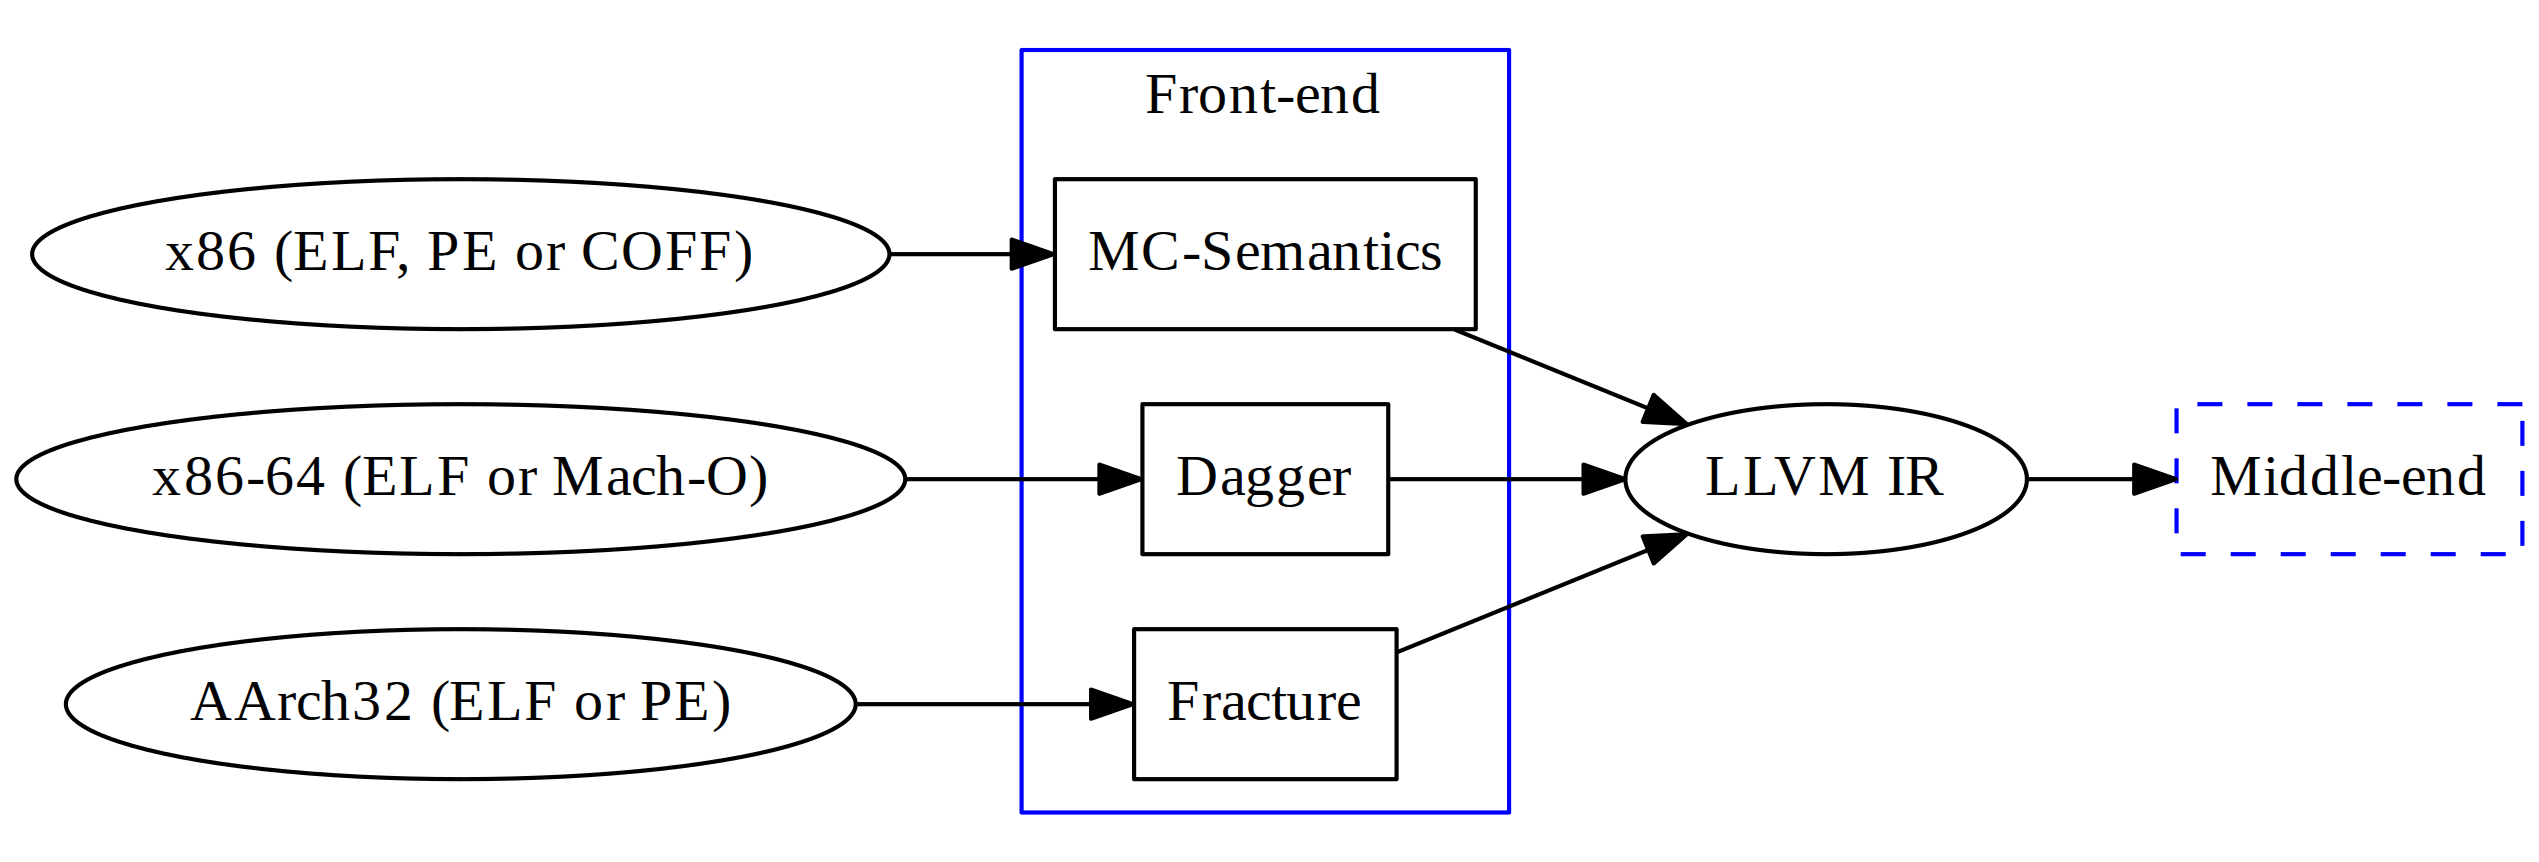
\includegraphics[width=\textwidth]{inc/6_design/front-end_binary.png}
		\caption{The three open source projects MC-Semantics, Dagger and Fracture translate native code of various architectures (e.g. x86, x86-64 and ARM) and file formats (e.g. ELF, PE, COFF and Mach-o) to LLVM IR.}
		\label{fig:front-end_binary}
	\end{center}
\end{figure}

% ~~~ [ Compilers ] ~~~~~~~~~~~~~~~~~~~~~~~~~~~~~~~~~~~~~~~~~~~~~~~~~~~~~~~~~~~~

\subsubsection{Compilers}
\label{sec:design_compilers}

One important aspect of utilizing the IR of a compiler framework, is that the decompilation pipeline automatically gains support for transpilation (i.e. translating one programming language into another) in addition to reverse compilation. An increasing number of open source compilers (e.g. Clang, GHC, \texttt{rustc}) are capable of translating a range of source languages (e.g. C, Haskell, Rust) into LLVM IR. These compilers may be used as-is by the front-end module (see figure \ref{fig:front-end_source}), thereby extending the supported source languages of the decompilation pipeline. Using this approach, the decompilation pipeline may translate $ n $ source languages into $ m $ target languages by implementing $ n + m $ front-end and back-end modules, instead of $ n \cdot m $ transpilers.

\begin{figure}[htbp]
	\begin{center}
		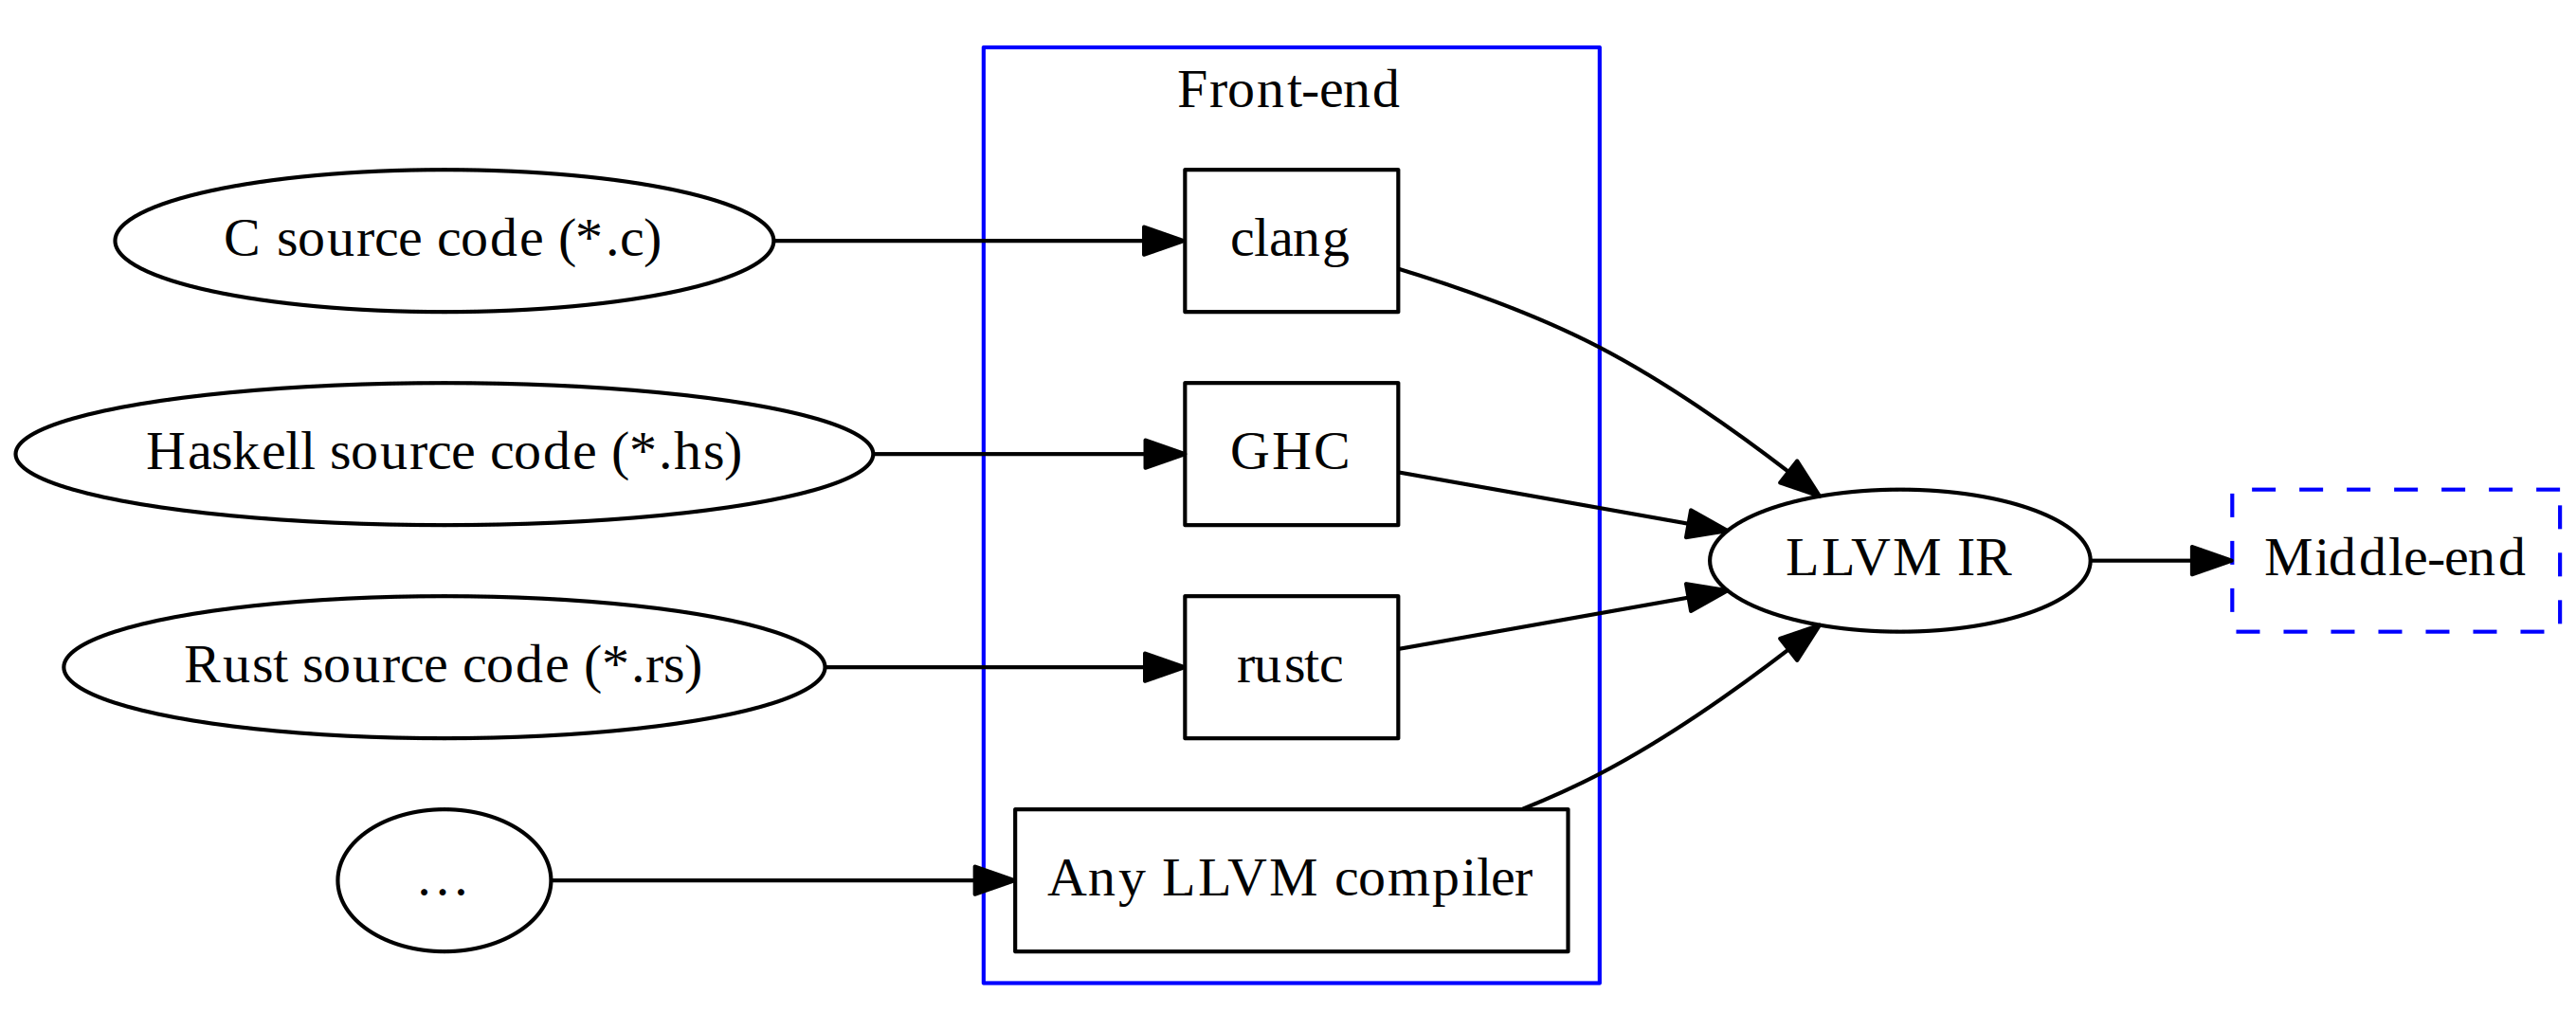
\includegraphics[width=\textwidth]{inc/6_design/front-end_source.png}
		\caption{Several open source compilers translate high-level programming languages into LLVM IR. Three such compilers are Clang, the Glasgow Haskell Compiler and the Rust compiler which translate C, Haskell and Rust respectively into LLVM IR.}
		\label{fig:front-end_source}
	\end{center}
\end{figure}

Another important aspect of utilizing LLVM IR, is that a wide range of optimizations have been implemented already by the LLVM compiler framework. This allows the front-end components to focus on translating the source languages into LLVM IR, without having to worry about producing highly optimised output. The LLVM IR may later be optimised by invoking the \texttt{opt} tool of LLVM to remove dead code, propagate constants, and promote memory accesses to registers, for instance.

